\chapter{Podstawy teoretyczne}

Rozdział obejmuje podstawy klasyfikacji niechcianej poczty za pomocą modeli
językowych. Opisano reprezentację i tokenizację tekstu, metryki klasyfikacji,
działanie modeli przyczynowych oraz architekturę Transformer. Następne sekcje
dotyczą dostrajania metodą LoRA, sposobów użycia modelu jako klasyfikatora oraz
kosztu treningu i inferencji.

% Cel rozdziału: wyjaśnić pojęcia potrzebne do zrozumienia części badawczej,
% bez opisywania decyzji eksperymentalnych i wyników z rozdziału badawczego.
% Konkretne wybory modelu, zbiorów danych, parametrów treningu i wyników
% powinny pozostać w rozdziale badawczym.

\section{Niechciana poczta elektroniczna}

\subsection{Pojęcie spamu}

W odniesieniu do poczty elektronicznej spam oznacza niechcianą wiadomość
wysyłaną masowo przez nadużycie systemów komunikacji elektronicznej~\autocite{nist-csrc-spam-glossary}.
Pod tą nazwą mieszczą się jednak wiadomości
o różnym celu i poziomie ryzyka. W korpusach spamowych pojawiają się
między innymi reklamy, próby oszustwa, phishing oraz fałszywe
informacje~\autocite{janez-martino-spam-topic-2024}. W zadaniu klasyfikacji
binarnej takie wiadomości są zwykle sprowadzane do jednej klasy niepożądanej.

\subsection{Typy niepożądanych wiadomości}

\subsubsection{Spam reklamowy}

Spam reklamowy służy przede wszystkim promowaniu produktu, usługi albo strony
internetowej. Wiadomości zazwyczaj są uciążliwe i prowadzą do zaśmiecania skrzynki
pocztowej. Reklamowany produkt bywa niskiej jakości,
niezgodny z opisem, fałszywy albo szkodliwy dla odbiorcy. Dotyczy to zwłaszcza
ofert leków, suplementów, usług finansowych, inwestycji lub produktów
obiecujących szybki efekt.

\subsubsection{Phishing}

Phishing polega na pozyskaniu wrażliwych danych, na przykład danych logowania
lub numerów kart płatniczych, przez podszycie się pod zaufaną firmę albo
instytucję~\autocite{nist-csrc-phishing-glossary}. W poczcie elektronicznej
atakujący najczęściej próbuje skłonić odbiorcę do kliknięcia linku, otwarcia
załącznika albo wpisania danych na fałszywej stronie. Adres takiej strony może
różnić się od prawdziwej witryny tylko pojedynczym znakiem, a jej wygląd może
naśladować oryginalny serwis. Po przejęciu danych atakujący może przekierować
użytkownika na prawdziwą stronę, aby zasymulować prawidłowe logowanie i nie
wzbudzić podejrzeń. Dla zwiększenia skuteczności wiadomości phishingowe często
wykorzystują elementy psychologiczne, takie jak presja czasu. Przykładem jest
wiadomość podszywająca się pod InPost, opisana przez Bitdefender w 2024
roku~\autocite{bitdefender-inpost-phishing-2024}:

\begin{framed}
\begin{displayquote}
\small\ttfamily\raggedright
INPOST: Masz paczkę 
INPOST, która dotarła do
stacji wysyłkowej, ale nie
może zostać dostarczona
ze względu na
nieprawidłowe dane
adresowe. Aby ułatwić
dostawę, zaktualizuj
informacje o dostawie tak
szybko, jak to możliwe. Aby
wprowadzić zmiany, otwórz
link do pakietu: \textit{[złośliwy link]}
\end{displayquote}
\end{framed}


\subsubsection{Wiadomości oszukańcze}

Wiadomości oszukańcze (ang. \emph{scam}) opierają się przede wszystkim na
inżynierii społecznej. Atakujący przyjmuje fałszywą tożsamość i próbuje
doprowadzić do sytuacji, w której odbiorca sam poda wrażliwe dane albo przekaże
pieniądze. Początkowo atak przypomina phishing, ale potem przechodzi w bezpośrednią rozmowę z oszustem.
Manipulacja nie musi nastąpić od razu. W niektórych wariantach kontakt trwa wiele dni lub tygodni,
a kolejne wiadomości stopniowo budują zaufanie~\autocite{advance-fee-fraud}.

W niniejszej pracy analizowane są wiadomości tekstowe, choć sam tekst może być
tylko jednym elementem oszustwa. Upowszechnienie narzędzi AI umożliwia atakującym
generowanie fałszywych zdjęć, nagrań głosu, a nawet przeprowadzanie wideorozmów ze zmianą
wyglądu w czasie rzeczywistym. Takie techniki wzmacniają wiarygodność atakującego i przyspieszają
zdobywanie zaufania ofiary~\autocite{pedersen-deepfake-social-engineering-2025}.

\subsection{Klasyfikacja wiadomości jako problem binarny}

W tej pracy filtrowanie poczty traktowane jest jako klasyfikacja binarna:
wiadomość może należeć do klasy korespondencji pożądanej albo do klasy
\emph{spam}, obejmującej spam reklamowy, phishing i wiadomości
oszukańcze. Taki zapis odpowiada decyzji filtra poczty: przepuścić wiadomość albo 
oznaczyć ją jako niepożądaną. Przy ocenie modelu ważny jest więc nie tylko odsetek poprawnych decyzji, lecz także
typ błędu. Błąd fałszywie dodatni (ang. \emph{false positive}, FP) oznacza
przeniesienie poprawnej wiadomości do spamu. Błąd fałszywie ujemny (ang.
\emph{false negative}, FN) oznacza przepuszczenie wiadomości niepożądanej do
skrzynki odbiorczej.

\section{Klasyfikacja tekstu}

\subsection{Reprezentacja dokumentu tekstowego}

W klasyfikacji tekstu dokument otrzymuje etykietę określającą jego klasę. Dla
wiadomości e-mail takim dokumentem może być sam temat, sama treść albo połączenie
obu pól. Metadane, nagłówki i informacje techniczne są szczególnie użyteczne, ale w
publicznych korpusach rzadko mają jednolity format. Celem pracy jest również
przeanalizowanie skuteczności wykrywania spamu na podstawie samego tekstu.

Model nie przetwarza jednak tekstu w takiej postaci, w jakiej widzi go
użytkownik. W klasycznych metodach uczenia maszynowego wiadomość zamienia się
zwykle na wektor cech, na przykład zliczenia słów albo wagi TF-IDF
~\autocite{janez-martino-spam-topic-2024}. W modelach językowych wejściem jest
sekwencja identyfikatorów tokenów.

Poczta elektroniczna jest pod tym względem mniej regularna niż typowy akapit
tekstu. Wiadomość może zawierać cytowaną korespondencję, podpis, linki, fragmenty
HTML, automatyczne stopki albo artefakty kodowania. Część tych elementów pomaga
w klasyfikacji, a część wprowadza szum. Przygotowanie danych wymaga więc decyzji,
które fragmenty wiadomości tworzą wejście modelu i jak traktować elementy
występujące tylko w niektórych zbiorach.

\subsection{Tokenizacja i długość kontekstu}

\subsubsection{Tokeny}

Token jest podstawową jednostką tekstu przetwarzaną przez model językowy. W
zależności od użytego tokenizatora może odpowiadać całemu słowu, fragmentowi
słowa, znakowi interpunkcyjnemu, części adresu URL albo tokenowi specjalnemu.
Dlatego długość wiadomości mierzona w tokenach różni się od długości mierzonej w
słowach. Link, nazwa domeny, nietypowy zapis kwoty albo celowo zniekształcone
słowo mogą zostać podzielone na wiele elementów.

Ma to znaczenie szczególnie dla spamu i phishingu. Takie wiadomości często
zawierają adresy URL, losowe ciągi znaków, nazwy domen, kwoty, daty i nietypowe
formatowanie. Dwie wiadomości o podobnej liczbie słów mogą więc po tokenizacji
mieć różną długość. Różnica ta wpływa później na koszt przetwarzania i na to,
czy cała treść mieści się w wejściu modelu.

\subsubsection{Tokenizacja BPE}

Byte Pair Encoding (BPE) jest algorytmem tworzenia tokenów przez łączenie
często występujących obok siebie fragmentów tekstu. Na początku tekst jest
reprezentowany jako krótkie jednostki, na przykład znaki albo bajty. Następnie
algorytm znajduje najczęstsze pary sąsiednich jednostek i dodaje ich połączenia
do słownika. Po wielu takich krokach częste fragmenty tekstu stają się
pojedynczymi tokenami, a rzadsze pozostają zapisane jako kilka krótszych
jednostek~\autocite{sennrich-subword-2016}.

\paragraph{Przykład tokenizacji byte-level BPE na podstawie GPT-2}

Jest to przykład dydaktyczny; w eksperymentach użyto tokenizatora Qwen3, który
ma własny słownik i reguły tokenizacji. Tokenizer GPT-2 wybrano do opisu,
ponieważ jego implementacja jest stosunkowo prosta i publicznie dostępna.
Nowsze modele często stosują bardziej rozbudowane wyrażenia regularne,
dodatkowe tokeny specjalne oraz implementacje, których pełny przebieg trudniej
odtworzyć wyłącznie z opisu modelu.

GPT-2 wykorzystywał wariant bajtowy BPE~\autocite{radford-gpt2-2019}. Tokenizer
działa w trzech głównych krokach:

\begin{enumerate}
    \item \textbf{Podział tekstu na fragmenty.} Wejściowy tekst jest dzielony za
    pomocą wyrażenia regularnego. W implementacji GPT-2 użyto następującego
    wzorca~\autocite{openai-gpt2-encoder}:

    \begin{lstlisting}[basicstyle=\small\ttfamily,breaklines=true,numbers=none]
's|'t|'re|'ve|'m|'ll|'d| ?\p{L}+| ?\p{N}+| ?[^\s\p{L}\p{N}]+|\s+(?!\S)|\s+
    \end{lstlisting}

    Dla tekstu \texttt{I've made a calculation! 3+3=6!!} taki podział daje
    fragmenty:

    \begin{lstlisting}[basicstyle=\small\ttfamily,breaklines=true,numbers=none]
['I', "'ve", ' made', ' a', ' calculation', '!', ' 3', '+', '3', '=', '6', '!!']
    \end{lstlisting}

    Zastosowanie takiego wyrażenia nie jest optymalne pod względem kompresji
    tekstu, ale ogranicza tworzenie tokenów łączących przypadkowe kombinacje
    liter, cyfr i interpunkcji. W opisie GPT-2 wskazano, że bez takiego
    ograniczenia BPE tworzyło wiele wariantów tych samych częstych słów, przez
    co gorzej wykorzystywało ograniczony słownik i pojemność
    modelu~\autocite{radford-gpt2-2019}.

    \item \textbf{Konwersja na bajty.} Każdy fragment jest zapisywany jako
    sekwencja bajtów UTF-8. Zbiór 256 wartości bajtowych tworzy bazowy słownik
    tokenizatora. Reprezentacja bajtowa pozwala zakodować każdy tekst w UTF-8
    bez potrzeby wprowadzania osobnego tokenu dla każdego znaku Unicode i bez
    tokenu nieznanego dla znaków spoza słownika, na przykład \texttt{<unk>}.
    Unicode przypisuje znakom abstrakcyjne punkty kodowe, natomiast UTF-8
    zapisuje je jako ciągi bajtów. Przykładowo
    znak \texttt{U+1F40E} jest reprezentowany w UTF-8 przez cztery bajty:
    \texttt{[240, 159, 144, 142]}. Tokenizer nie potrzebuje więc osobnego wpisu
    dla każdego znaku Unicode, ponieważ może zapisać go za pomocą elementów
    bazowego słownika bajtowego.

    \item \textbf{Zastosowanie reguł BPE.} Na reprezentacji bajtowej stosowane są
    reguły BPE wyuczone wcześniej na korpusie tekstowym. Częste sąsiednie ciągi
    bajtów są łączone w dłuższe tokeny, a rzadsze fragmenty pozostają rozbite na
    krótsze jednostki. Podczas inferencji i treningu tokenizer stosuje gotowy słownik i
    listę połączeń.
\end{enumerate}

Kolejne etapy tokenizacji zestawiono na
rysunku~\ref{fig:bpe-tokenization-gpt2}.

\begin{figure}[H]
\centering
\resizebox{\textwidth}{!}{\begingroup
\begin{tikzpicture}[
    >=Stealth,
    font=\sffamily,
    stage/.style={rounded corners=5pt, draw=plotBlue!50, fill=plotBlue!5,
        line width=0.8pt, minimum width=12.35cm, minimum height=1.02cm,
        align=center},
    chip/.style={rounded corners=2pt, draw=black!25, fill=white,
        minimum height=0.48cm, inner xsep=5pt, align=center, font=\scriptsize},
    byte/.style={rounded corners=2pt, draw=plotAccent!45, fill=plotAccent!8,
        minimum height=0.48cm, inner xsep=4pt, align=center, font=\scriptsize},
    merge/.style={rounded corners=2pt, draw=plotHam!45, fill=plotHam!8,
        minimum height=0.48cm, inner xsep=4pt, align=center, font=\scriptsize},
    arrow/.style={->, draw=black!55, line width=0.8pt},
    small/.style={font=\scriptsize, text=black!70, align=center},
    title/.style={font=\tiny\bfseries, text=black!85, align=center}
]

\path[use as bounding box] (-0.15,-3.85) rectangle (12.60,3.95);

\foreach \name/\y in {
    input/3.25,
    regex/1.75,
    bytes/0.25,
    bpe/-1.25,
    ids/-2.75
} {
    \node[stage] (\name) at (6.20,\y) {};
    \draw[black!15, line width=0.5pt] (2.80,\y-0.41) -- (2.80,\y+0.41);
}

\node[title] at (1.47,3.25) {\shortstack{Tekst\\wejściowy}};
\node[title] at (1.47,1.75) {\shortstack{1. Podział\\wyrażeniem\\regularnym}};
\node[title] at (1.47,0.25) {\shortstack{2. Bajty\\UTF-8}};
\node[title] at (1.47,-1.25) {\shortstack{3. Reguły\\BPE}};
\node[title] at (1.47,-2.75) {Identyfikatory};

% Komórki w wierszach są układane w stałym obszarze x=3.55..10.95.
% Dzięki temu rozkład przypomina space-between i nie zależy od długości podpisu.
\node[chip, minimum width=4.10cm, fill=plotBlue!8] at (7.25,3.25)
    {\texttt{Lorem ipsum dolor sit amet}};

\node[chip] at (3.75,1.75) {\texttt{Lorem}};
\node[chip] at (5.50,1.75) {$\sqcup$\texttt{ipsum}};
\node[chip] at (7.25,1.75) {$\sqcup$\texttt{dolor}};
\node[chip] at (9.00,1.75) {$\sqcup$\texttt{sit}};
\node[chip] at (10.65,1.75) {$\sqcup$\texttt{amet}};

\node[byte, anchor=west, minimum width=3.25cm] at (3.55,0.25)
    {\texttt{Lorem} $\rightarrow$ \texttt{76 111 ...}};
\node[byte, anchor=east, minimum width=3.25cm] at (10.95,0.25)
    {$\sqcup$\texttt{ipsum} $\rightarrow$ \texttt{32 105 ...}};

\node[merge, anchor=west, minimum width=1.50cm] at (3.55,-1.25)
    {\texttt{L}+\texttt{o} $\rightarrow$ \texttt{Lo}};
\node[merge, minimum width=1.70cm] at (6.48,-1.25)
    {\texttt{Lo}+\texttt{r} $\rightarrow$ \texttt{Lor}};
\node[merge, anchor=east, minimum width=3.00cm] at (10.95,-1.25)
    {\texttt{...} $\rightarrow$ dłuższe tokeny};

\node[chip, fill=plotHam!8, anchor=west, minimum width=2.00cm] at (3.55,-2.75)
    {\texttt{Lorem} $\rightarrow$ $id_1$};
\node[chip, fill=plotHam!8, minimum width=2.00cm] at (7.25,-2.75)
    {$\sqcup$\texttt{ipsum} $\rightarrow$ $id_2$};
\node[chip, fill=plotHam!8, anchor=east, minimum width=2.00cm] at (10.95,-2.75)
    {$\ldots$ $\rightarrow$ $id_n$};

% Strzałki są centrowane względem prawej części wierszy, a nie całego pola z etykietą.
\draw[arrow] (7.25,2.74) -- (7.25,2.26);
\draw[arrow] (7.25,1.24) -- (7.25,0.76);
\draw[arrow] (7.25,-0.26) -- (7.25,-0.74);
\draw[arrow] (7.25,-1.76) -- (7.25,-2.24);

\node[small, anchor=west] at (0.20,-3.55)
    {$\sqcup$ oznacza spację poprzedzającą fragment tekstu.};

\end{tikzpicture}
\endgroup
}
\caption[Przykład tokenizacji byte-level BPE na podstawie GPT-2]{Przykład
tokenizacji byte-level BPE na podstawie GPT-2. Jest to przykład dydaktyczny
przedstawiający trzy etapy tokenizacji tekstu \texttt{Lorem ipsum dolor sit
amet}. W eksperymentach użyto tokenizatora Qwen3, który ma własny słownik i
reguły tokenizacji.}
\label{fig:bpe-tokenization-gpt2}
\figuresource{opracowanie własne.}
\end{figure}

\subsubsection{Długość kontekstu}

Maksymalna długość wejścia modelu nazywana jest oknem kontekstu. Gdy wiadomość
po tokenizacji przekracza ten limit, konieczne jest jej obcięcie. Skracanie
może usunąć ważny fragment, na przykład link umieszczony pod koniec treści.
Dłuższe okno kontekstu zachowuje więcej informacji, ale zwiększa koszt treningu
i inferencji. W praktyce długość wejścia jest więc kompromisem między ilością
zachowanego tekstu a kosztem obliczeniowym.

\subsection{Metryki oceny klasyfikatora}

W problemach binarnych, takich jak klasyfikacja korespondencji, podstawowym elementem ewaluacji modelu jest macierz pomyłek.
Przedstawia ona cztery możliwe kombinacje klasyfikacji.
W tej pracy klasą pozytywną jest spam, phishing lub inna wiadomość niepożądana, a klasą negatywną pożądana korespondencja.
Znaczenie jej pól przedstawiono w tabeli~\ref{tab:confusion-matrix}.

\begin{table}[H]
    \centering
    \caption{Macierz pomyłek dla binarnej klasyfikacji wiadomości}
    \label{tab:confusion-matrix}
    \renewcommand{\arraystretch}{1.25}
    \begin{tabular}{
    |>{\centering\arraybackslash}m{0.24\linewidth}
    |>{\centering\arraybackslash}m{0.31\linewidth}
    |>{\centering\arraybackslash}m{0.31\linewidth}|}
    \hline
    & \textbf{Rzeczywista wiadomość niepożądana}
    & \textbf{Rzeczywista wiadomość pożądana} \\
    \hline
    \textbf{Wiadomość przewidziana jako niepożądana}
    & \shortstack[c]{\\[0.2em]{\textbf{TP}}\\[0.2em]\small\emph{True positive}\\\small Poprawnie wykryty spam}
    & \shortstack[c]{\\[0.2em]{\textbf{FP}}\\[0.2em]\small\emph{False positive}\\\small Pożądana wiadomość\\\small oznaczona jako spam} \\
    \hline
    \textbf{Wiadomość przewidziana jako pożądana}
    & \shortstack[c]{\\[0.2em]{\textbf{FN}}\\[0.2em]\small\emph{False negative}\\\small Spam przepuszczony\\\small jako wiadomość pożądana}
    & \shortstack[c]{\\[0.2em]{\textbf{TN}}\\[0.2em]\small\emph{True negative}\\\small Poprawnie rozpoznana\\\small wiadomość pożądana} \\
    \hline
\end{tabular}

\end{table}

\emph{Accuracy} podaje udział poprawnych decyzji w całym zbiorze:

\[
\mathrm{accuracy} =
\frac{TP + TN}{TP + TN + FP + FN}.
\]

Przy nierównych klasach samo \emph{accuracy} może ukrywać problemy z
rozpoznawaniem klasy rzadszej. Model wybierający głównie klasę większościową
nadal może osiągnąć wysoki wynik, mimo że przepuszcza wiele przykładów drugiej
klasy. Dlatego obok tej metryki stosuje się miary opisujące osobno decyzje dla
spamu i wiadomości pożądanych.

\emph{Precision} określa, jaki odsetek wiadomości oznaczonych przez model jako
spam rzeczywiście należał do tej klasy:

\[
\mathrm{precision} =
\frac{TP}{TP + FP}.
\]

\emph{Recall} pokazuje, jaki odsetek rzeczywistych wiadomości spamowych został
wykryty:

\[
\mathrm{recall} =
\frac{TP}{TP + FN}.
\]

\emph{Specificity} pełni podobną rolę dla klasy negatywnej. Mierzy odsetek
wiadomości pożądanych, których model nie oznaczył jako spam:

\[
\mathrm{specificity} =
\frac{TN}{TN + FP}.
\]

F1 jest średnią harmoniczną \emph{precision} i \emph{recall}:

\[
F1 =
2 \cdot \frac{\mathrm{precision} \cdot \mathrm{recall}}
{\mathrm{precision} + \mathrm{recall}}.
\]

F1 łączy \emph{precision} i \emph{recall} klasy pozytywnej. Niska wartość jednej
z tych składowych mocno obniża wynik, dlatego metryka nie premiuje modeli dobrych
tylko w jednym z tych aspektów. Nie uwzględnia jednak liczby poprawnie
rozpoznanych przykładów klasy negatywnej, dlatego powinna być interpretowana
razem z \emph{specificity}, FPR oraz rozkładem klas.

\emph{Balanced accuracy} uśrednia \emph{recall} i \emph{specificity}, więc w
równym stopniu uwzględnia klasę pozytywną i negatywną:

\[
\mathrm{balanced\ accuracy} =
\frac{\mathrm{recall} + \mathrm{specificity}}{2}.
\]


\section{Modele językowe}

\subsection{Zadanie modelowania języka}

Model językowy opisuje prawdopodobieństwo sekwencji tokenów. Dla tekstu
zapisanego jako \(x_1, x_2, \ldots, x_n\) oznacza to ocenę, jak prawdopodobna
jest dana kolejność elementów języka. Taka definicja jest użyteczna także wtedy,
gdy interesuje nas nie prawdopodobieństwo całego tekstu, lecz brakujący albo
kolejny fragment. Model uczy się bowiem zależności między tokenami
występującymi w korpusie
~\autocite{bengio-neural-probabilistic-language-model}.

Współczesny model językowy przechodzi najpierw trening na dużym
zbiorze tekstu, bez etykiet przygotowanych dla jednego zadania. Uczy się wtedy
składni, typowych związków między słowami, sposobów zapisu informacji oraz
części regularności obecnych w danych treningowych. Dopiero później taki model
można dostosować do konkretnego problemu, na przykład do rozróżniania wiadomości
\texttt{spam} i \texttt{ham}. Nie oznacza to trenowania modelu od początku.
Zwykle wystarcza dalsze uczenie na mniejszym korpusie zadaniowym.

W tej pracy model językowy zastępuje ręcznie zaprojektowany wektor cech opisany
we wcześniejszej części rozdziału. Wiadomość jest zamieniana na sekwencję
tokenów, a model wykorzystuje reprezentacje wyuczone podczas pretrainingu.
Część badawcza sprawdza, jak skutecznie takie reprezentacje da się dostroić do wykrywania
niepożądanej korespondencji.

\subsection{Modele przyczynowe i przewidywanie następnego tokenu}

W modelowaniu przyczynowym (ang. \emph{causal language modeling}) model otrzymuje
wcześniejsze tokeny i na ich podstawie przewiduje następny. Nie korzysta z
informacji po prawej stronie przewidywanej pozycji, więc zależność odpowiada
generowaniu tekstu od lewej do prawej. Dla sekwencji \(x_1, \ldots, x_n\)
prawdopodobieństwo tekstu zapisuje się jako iloczyn prawdopodobieństw kolejnych
tokenów:

\[
P(x_1, \ldots, x_n) =
\prod_{i=1}^{n} P(x_i \mid x_1, \ldots, x_{i-1}).
\]

Taki sposób uczenia wykorzystano między innymi w rodzinie modeli GPT
~\autocite{radford-gpt2-2019,brown-language-models-few-shot}. Podczas generowania
model zwraca rozkład prawdopodobieństwa nad słownikiem tokenizatora. Z tego
rozkładu można wybrać najbardziej prawdopodobny token albo próbkować tokeny z
uwzględnieniem parametrów dekodowania. Ten sam rozkład może posłużyć do
klasyfikacji.

W zadaniu binarnym prompt można ułożyć tak, aby następnym oczekiwanym elementem
była etykieta klasy. Model nie generuje wtedy pełnej odpowiedzi. Wystarczy
porównać prawdopodobieństwa tokenów odpowiadających etykietom \texttt{spam} i
\texttt{ham}. Decyzja klasyfikatora wynika z rozkładu prawdopodobieństwa w
jednej pozycji, a nie z późniejszego parsowania tekstu zwróconego przez model.
Takie podejście zależy jednak od tokenizacji etykiet oraz od sformułowania
promptu. Jeżeli etykieta składa się z wielu tokenów albo prompt kieruje model w
stronę innej odpowiedzi, porównanie staje się mniej jednoznaczne.

\subsection{Modele instrukcyjne i format czatu}

Sam pretraining uczy model przewidywania tekstu, ale nie gwarantuje, że model
będzie wykonywał polecenia użytkownika w przewidywalnym formacie. Modele, z
którymi zazwyczaj mamy kontakt, przechodzą więc dodatkowe dostrajanie
instrukcyjne (ang. \emph{instruction tuning}). Dane treningowe mają wtedy postać instrukcji i
oczekiwanej odpowiedzi, a celem jest dopasowanie zachowania modelu do poleceń
podawanych wprost przez użytkownika. W praktyce etap ten może być łączony z
uczeniem z informacji zwrotnej od ludzi~\autocite{ouyang-instruction-following}.

Modele instrukcyjne często pracują w formacie czatu. Zamiast pojedynczego ciągu
tekstu wejście składa się z komunikatów o rolach. Najczęściej spotykane role to
\texttt{system}, \texttt{user} i \texttt{assistant}. Komunikat systemowy
określa ogólne zachowanie modelu, komunikat użytkownika zawiera polecenie, a
odpowiedź asystenta jest tekstem generowanym przez model. W treści komunikatu
asystenta mogą występować dodatkowe bloki, na przykład \texttt{think} służący
do zapisu rozumowania lub \texttt{tool\_call} opisujący wywołanie narzędzia.
Przed przekazaniem danych do modelu komunikaty
są zamieniane na sekwencję tokenów według szablonu czatu, który dodaje
znaczniki ról i tokeny specjalne.

Schemat poglądowy takiej rozmowy, oparty na składni ChatML, pokazuje
listing~\ref{lst:chatml-weather-template}~\autocite{qwen3-06b-model-card}.

\begin{lstlisting}[
    basicstyle=\ttfamily\footnotesize,
    breaklines=true,
    numbers=none,
    caption={Schemat poglądowy rozmowy w stylu ChatML z blokiem analizy i wywołaniem narzędzia.},
    label={lst:chatml-weather-template}
]
<|im_start|>system
You are a weather assistant. Answer weather questions briefly.
# Tools
<tools>
{"type": "function", "function": {"name": "get_weather", "description": "Get weather for a city", "parameters": {"type": "object", "properties": {"city": {"type": "string"}, "unit": {"type": "string"}}, "required": ["city"]}}}
</tools>
Return each function call as JSON inside <tool_call></tool_call>.
<|im_end|>
<|im_start|>user
What is the weather in Tokyo?<|im_end|>
<|im_start|>assistant
<think>
I need to check the weather for Tokyo.
</think>
I will check the weather in Tokyo.
<tool_call>
{"name": "get_weather", "arguments": {"city": "Tokyo", "unit": "celsius"}}
</tool_call><|im_end|>
<|im_start|>user
<tool_response>
{"temperature": 22, "condition": "partly cloudy"}
</tool_response><|im_end|>
<|im_start|>assistant
Tokyo is 22 degrees Celsius and partly cloudy.<|im_end|>
\end{lstlisting}

W klasyfikacji wiadomości taki format sprowadza zadanie do instrukcji:
oceń treść wiadomości i zwróć jedną z dwóch etykiet.
Pozostaje jednak problem kontroli odpowiedzi. Zamiast samego słowa
\texttt{spam} model może wygenerować pełne zdanie, uzasadnienie albo odpowiedź w
niepełnym formacie. Metody oparte na generowaniu wymagają więc parsera, który
zamienia tekst odpowiedzi na etykietę. Metoda przewidywania następnego tokenu
ogranicza ten problem, ponieważ porównuje prawdopodobieństwa etykiet przed
wygenerowaniem dłuższej odpowiedzi.

Model instrukcyjny nadal trzeba dopasować do zadania, ale daje praktyczny punkt
startowy. Rozpoznaje strukturę polecenia, pracuje w formacie czatu i
może zostać dalej dostrojony na przykładach zawierających wiadomości e-mail oraz
oczekiwane etykiety. Ta własność jest później wykorzystywana przy porównaniu
testowanych wariantów klasyfikacji: klasyfikacji sekwencji, generowania etykiety,
przewidywania następnego tokenu oraz generowania odpowiedzi strukturyzowanej.

\pagebreak

\section{Architektura Transformer}

Architektura Transformer~\autocite{vaswani-attention-is-all-you-need} składa się
z powtarzanych bloków, które przetwarzają reprezentacje kolejnych pozycji
sekwencji. Po tokenizacji identyfikatory tokenów są zamieniane na wektory. Do
wektorów dodaje się informację o położeniu tokenu w tekście, a następnie cała
sekwencja przechodzi przez kolejne bloki Transformera. Każdy blok aktualizuje
opis danej pozycji na podstawie jej dotychczasowej postaci oraz kontekstu
pozostałych tokenów.

Wariant decoder-only, używany w wielu generatywnych modelach językowych, działa
przyczynowo: na podstawie wcześniejszych tokenów oblicza rozkład
prawdopodobieństwa następnego tokenu. Pojedynczy blok łączy mechanizm
self-attention z siecią feed-forward. Pierwszy element wiąże informacje z różnych
pozycji sekwencji, a drugi przekształca reprezentację każdej pozycji osobno. W
praktycznych implementacjach stosuje się także normalizację warstw i połączenia
rezydualne, które stabilizują przepływ informacji przez wiele warstw
modelu~\autocite{vaswani-attention-is-all-you-need}.

Ogólny przebieg danych przez model decoder-only przedstawiono na
rysunku~\ref{fig:transformer-overview}.

\begin{figure}[p]
\centering
\resizebox{!}{0.77\textheight}{\begingroup
\begin{tikzpicture}[
    >=Stealth,
    font=\sffamily,
    token/.style={rounded corners=2pt, draw=black!25, fill=plotBlue!8,
        minimum width=1.75cm, minimum height=0.62cm, align=center,
        font=\small},
    emb/.style={rounded corners=2pt, draw=plotBlue!45, fill=plotBlue!10,
        minimum width=1.55cm, minimum height=0.50cm},
    transformer/.style={rounded corners=6pt, draw=plotAccent!60,
        fill=plotAccent!5, line width=0.9pt, minimum width=10.6cm,
        minimum height=4.2cm},
    subblock/.style={rounded corners=4pt, draw=plotAccent!55, fill=white,
        line width=0.75pt, minimum width=3.2cm, minimum height=1.05cm,
        align=center, font=\small},
    stage/.style={rounded corners=5pt, draw=plotBlue!45, fill=plotBlue!5,
        line width=0.75pt, minimum width=4.0cm, minimum height=1.0cm,
        align=center},
    arrow/.style={->, draw=black!60, line width=0.75pt},
    flow/.style={->, draw=plotBlue!75, line width=0.9pt},
    small/.style={font=\scriptsize, text=black!70, align=center},
    heading/.style={font=\small\bfseries, align=center}
]

\path[use as bounding box] (-6.0,-6.35) rectangle (6.0,11.15);

% Tokeny wejściowe.
\node[heading] at (0,10.70) {Tokeny};
\foreach \word/\name/\x in {
    Lorem/tok1/-4.0,
    ipsum/tok2/-2.0,
    dolor/tok3/0,
    sit/tok4/2.0,
    amet/tok5/4.0
} {
    \node[token] (\name) at (\x,9.95) {\texttt{\word}};
}

% Reprezentacje tokenów wraz z informacją o pozycji.
\foreach \name/\x in {emb1/-4.0,emb2/-2.0,emb3/0,emb4/2.0,emb5/4.0} {
    \node[emb] (\name) at (\x,8.05) {};
    \foreach \dx in {-0.48,-0.24,0,0.24,0.48} {
        \draw[plotBlue!45, line width=0.35pt]
            ($(\name.center)+(\dx,-0.21)$) -- ++(0,0.42);
    }
}
\foreach \a/\b in {tok1/emb1,tok2/emb2,tok3/emb3,tok4/emb4,tok5/emb5} {
    \draw[arrow] (\a.south) -- (\b.north);
}
\node[heading, fill=white, inner xsep=7pt, inner ysep=2pt] at (0,8.95)
    {Wektory tokenów + pozycja};

% Stos bloków Transformera.
\node[transformer, fill=plotBlue!6] (tr4) at (0.48,4.47) {};
\node[transformer, fill=plotBlue!9] (tr3) at (0.32,4.63) {};
\node[transformer, fill=plotBlue!12] (tr2) at (0.16,4.79) {};
\node[transformer] (tr1) at (0,4.95) {};

\draw[flow] (emb3.south) -- (tr1.north);
\node[font=\bfseries, text=plotAccent!85] at (0,6.41)
    {Stos bloków Transformera};
\node[small] at (0,6.02)
    {każdy blok zawiera mechanizm attention oraz sieć feed-forward};

\node[subblock, fill=plotAccent!11] (attn3) at (-2.04,4.47) {};
\node[subblock, fill=plotAccent!16] (attn2) at (-2.20,4.63) {};
\node[subblock] (attn1) at (-2.36,4.79)
    {multi-head\\attention};
\node[subblock] (ffn) at (2.28,4.79)
    {feed-forward\\network};
\draw[flow] (attn1.east) -- (ffn.west);

% Warstwa wyjściowa.
\node[stage] (output) at (0,1.45) {warstwa liniowa + softmax};
\draw[flow] (tr1.south) -- (output.north);

% Rozkład prawdopodobieństwa następnego tokenu.
\node[heading, fill=white, inner xsep=6pt, inner ysep=2pt] at (0,0.15)
    {Prawdopodobieństwa następnego tokenu};
\draw[arrow] (output.south) -- (0,0.48);

\node[rounded corners=5pt, draw=black!20, fill=black!1,
    minimum width=10.6cm, minimum height=4.35cm] (probbox) at (0,-2.45) {};

\foreach \tok/\pct/\w/\y in {
    consectetur/42\%/3.35/-1.05,
    elit/27\%/2.15/-1.75,
    adipiscing/16\%/1.28/-2.45,
    sed/8\%/0.64/-3.15,
    do/7\%/0.56/-3.85
} {
    \node[font=\scriptsize, anchor=east] at (-2.25,\y) {\texttt{\tok}};
    \draw[plotGrid, line width=3.0pt] (-1.95,\y) -- (2.70,\y);
    \draw[plotAccent, line width=3.0pt] (-1.95,\y) -- ++(\w,0);
    \node[font=\scriptsize, anchor=west, text=black!70] at (2.95,\y) {\pct};
}

\node[small] at (0,-5.15)
    {Warstwa wyjściowa wyznacza rozkład nad słownikiem modelu.};

\end{tikzpicture}
\endgroup
}
\caption[Przepływ informacji w modelu opartym na architekturze Transformer]
{Uproszczony przepływ informacji w modelu językowym opartym na
architekturze Transformer dla sekwencji \texttt{Lorem ipsum dolor sit amet}.
}
\label{fig:transformer-overview}
\figuresource{opracowanie własne.}
\end{figure}

\subsection{Mechanizm self-attention}

Mechanizm self-attention jest jednym z podstawowych elementów architektury
Transformer. Wyznacza wagi relacji między tokenami w tej samej sekwencji, a
następnie wykorzystuje je do obliczenia nowej reprezentacji każdego tokenu. W
klasycznych modelach sekwencyjnych
informacja przechodziła zwykle krok po kroku przez kolejne pozycje. Transformer
pozwala natomiast każdej pozycji porównać własną reprezentację z reprezentacjami
innych pozycji w oknie kontekstu. Dzięki temu w jednej warstwie można powiązać
fragmenty wiadomości oddalone od siebie, na przykład nazwę nadawcy, link w
treści i późniejszą prośbę o wykonanie płatności.

Dla macierzy reprezentacji wejściowych \(X\) warstwa self-attention tworzy trzy
rzutowania liniowe: zapytania \(Q\), klucze \(K\) oraz wartości \(V\):

\[
Q = XW_Q,\qquad K = XW_K,\qquad V = XW_V.
\]

Zapytania określają, czego dana pozycja szuka w sekwencji. Klucze służą do
obliczenia dopasowania z innymi pozycjami, a wartości są wektorami, z których
powstaje nowa reprezentacja. Wagi uwagi wyznacza się przez porównanie zapytań z
kluczami. W wersji scaled dot-product attention ma to postać:

\[
\mathrm{Attention}(Q,K,V) =
\mathrm{softmax}\left(\frac{QK^T}{\sqrt{d_k}}\right)V,
\]

gdzie \(d_k\) oznacza wymiar wektorów kluczy. Iloczyn \(QK^T\) tworzy macierz
podobieństw między pozycjami, a funkcja \(\mathrm{softmax}\) zamienia te wartości
na wagi sumujące się do jedności. Warstwa zwraca ważoną sumę wektorów \(V\),
osobną dla każdej pozycji w sekwencji.

W modelach językowych generujących tekst self-attention jest uzupełniany maską
przyczynową. Maska blokuje dostęp do tokenów znajdujących się po prawej stronie
aktualnej pozycji. Model korzysta więc z wcześniejszego kontekstu, ale podczas
przewidywania następnego tokenu nie widzi przyszłych elementów sekwencji. Jest
to ten sam warunek, który wcześniej opisano przy modelowaniu przyczynowym.

Warstwa uwagi zwykle działa w wersji wielogłowej (ang. \emph{multi-head
attention}). Każda głowa ma własne rzutowania \(Q\), \(K\) i \(V\), a uzyskane
wyniki są później łączone. Wielogłowy mechanizm uwagi umożliwia modelowanie
różnych relacji; w tej pracy nie analizowano jednak funkcji poszczególnych głów.

Przykładowy przepływ danych między głowami uwagi pokazano na
rysunku~\ref{fig:multi-head-self-attention-recap}.

\begin{figure}[htbp]
\centering
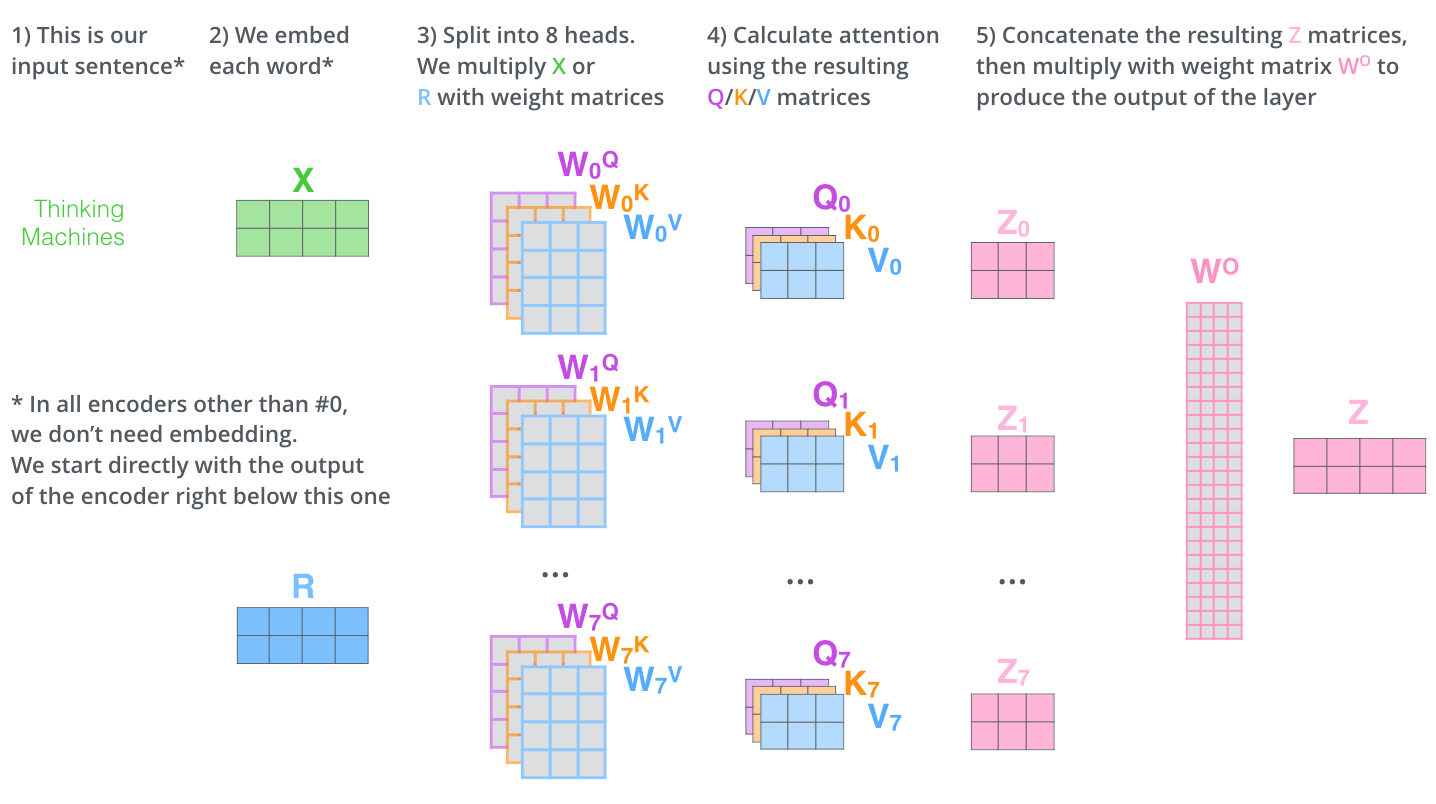
\includegraphics[width=\textwidth]{img/transformer_multi_headed_self_attention_recap}
\caption{Schemat działania mechanizmu multi-head self-attention.}
\label{fig:multi-head-self-attention-recap}
\figuresource{Jay Alammar, \emph{The Illustrated Transformer}
~\autocite{alammar-illustrated-transformer}.}
\end{figure}

\subsection{Okno kontekstu i koszt przetwarzania sekwencji}

Okno kontekstu określa maksymalną liczbę tokenów, które model przetwarza w
jednym przebiegu.

Do reprezentacji tokenów dodaje się informację o pozycji w sekwencji. W
oryginalnym Transformerze zastosowano sinusoidalne reprezentacje
pozycyjne~\autocite{vaswani-attention-is-all-you-need}. Nowsze modele mogą używać
innych sposobów kodowania pozycji. Informacja o pozycji pozwala modelowi
rozróżnić te same tokeny występujące w różnych miejscach tekstu.

W standardowym mechanizmie self-attention iloczyn \(QK^T\) dla sekwencji o
długości \(n\) tworzy macierz \(n \times n\), ponieważ warstwa uwagi porównuje
każdą pozycję z każdą inną pozycją w sekwencji. Przejście z 512 do 1024 tokenów
zwiększa rozmiar tej macierzy czterokrotnie. Część kosztu związana z macierzą
uwagi rośnie jak \(O(n^2)\); całkowity koszt zależy również od wymiaru ukrytego i
implementacji.

Koszt obsługi długiego kontekstu jest jedną z głównych barier w rozwoju modeli
językowych. Ograniczają go między innymi uwaga liniowa (ang. \emph{linear
attention}), uwaga rzadka (ang. \emph{sparse attention}), uwaga o stałym
wzorcu połączeń, warianty blokowe i blokowo-rzadkie oraz metody grupowania
tokenów~\autocite{sun-efficient-attention-survey}.


\subsection{Sieć feed-forward w bloku Transformer}

Po warstwie attention w każdym bloku Transformera znajduje się sieć
feed-forward (ang. \emph{feed-forward neural network}, FFN). Jej wejściem jest
reprezentacja tokenu po uwzględnieniu kontekstu przez attention. Ta sama para
przekształceń liniowych jest stosowana osobno dla każdej pozycji sekwencji:

\[
\mathrm{FFN}(x)=\sigma(xW_1+b_1)W_2+b_2.
\]

W oryginalnej architekturze Transformer funkcją \(\sigma\) była
ReLU~\autocite{vaswani-attention-is-all-you-need}; w nowszych modelach spotyka
się także inne aktywacje i warianty bramkowane. Układ pozostaje podobny:
pierwsze rzutowanie rozszerza wymiar wewnętrzny, aktywacja wprowadza
nieliniowość, a drugie rzutowanie sprowadza wynik z powrotem do wymiaru
używanego przez resztę modelu.

FFN przetwarza każdą pozycję osobno, ale korzysta z reprezentacji wzbogaconej
wcześniej przez attention. W bloku Transformer attention zbiera więc informacje
z sekwencji, a FFN wykonuje nieliniowe przekształcenie tej reprezentacji.
Schemat dwóch przekształceń liniowych przedstawiono na
rysunku~\ref{fig:feed-forward-network}.

\begin{figure}[H]
\centering
\begingroup
\centering
\begin{tikzpicture}[
    >=Stealth,
    neuron/.style={circle, draw=plotBlue, fill=plotBlue!10, minimum size=8mm, inner sep=0pt},
    hidden/.style={circle, draw=plotAccent, fill=plotAccent!12, minimum size=8mm, inner sep=0pt},
    output/.style={circle, draw=plotHam, fill=plotHam!12, minimum size=8mm, inner sep=0pt},
    conn/.style={->, draw=black!35, line width=0.35pt},
    mainconn/.style={->, draw=black!70, line width=0.7pt},
    label/.style={font=\small},
    smalllabel/.style={font=\scriptsize, align=center}
]

\foreach \y/\name/\lab in {1.1/i1/$x_1$,0/i2/$x_2$,-1.1/i3/$x_d$}
    \node[neuron] (\name) at (0,\y) {\lab};

\foreach \y/\name/\lab in {1.65/h1/$h_1$,0.55/h2/$h_2$,-0.55/h3/$h_3$,-1.65/h4/$h_m$}
    \node[hidden] (\name) at (3.2,\y) {\lab};

\foreach \y/\name/\lab in {1.1/o1/$y_1$,0/o2/$y_2$,-1.1/o3/$y_d$}
    \node[output] (\name) at (6.4,\y) {\lab};

\foreach \i in {i1,i2,i3}
    \foreach \h in {h1,h2,h3,h4}
        \draw[conn] (\i) -- (\h);

\foreach \h in {h1,h2,h3,h4}
    \foreach \o in {o1,o2,o3}
        \draw[conn] (\h) -- (\o);

\draw[mainconn] (-0.95,0) -- (i2);
\draw[mainconn] (o2) -- (7.35,0);

\node[label] at (0,2.35) {Wejście};
\node[label] at (3.2,2.35) {Warstwa ukryta};
\node[label] at (6.4,2.35) {Wyjście};

\node[smalllabel] at (0,-2.35) {$d_{\mathrm{model}}$};
\node[smalllabel] at (3.2,-2.35) {$d_{\mathrm{ff}}$};
\node[smalllabel] at (6.4,-2.35) {$d_{\mathrm{model}}$};

\node[smalllabel, fill=white, inner sep=2pt] at (1.6,1.95) {$W_1+b_1$};
\node[smalllabel, fill=white, inner sep=2pt] at (3.2,-2.85) {aktywacja $\sigma$};
\node[smalllabel, fill=white, inner sep=2pt] at (4.8,1.95) {$W_2+b_2$};

\node[smalllabel, anchor=east] at (-1.05,0) {$x$};
\node[smalllabel, anchor=west] at (7.45,0) {$\mathrm{FFN}(x)$};

\end{tikzpicture}
\endgroup

\caption{Uproszczony schemat sieci feed-forward typu MLP w bloku Transformera.}
\label{fig:feed-forward-network}
\figuresource{opracowanie własne.}
\end{figure}

\section{Dostrajanie modeli językowych}

\subsection{Fine-tuning}

Dostrajanie modelu (ang. \emph{fine-tuning}) polega na dalszym trenowaniu
modelu wstępnie trenowanego na danych związanych z konkretnym zadaniem. Model nie
jest wtedy uczony od początku. Punkt wyjścia stanowią parametry uzyskane podczas
pretrenowania, a trening zadaniowy przesuwa zachowanie modelu w stronę danych,
formatu odpowiedzi i kryterium oceny potrzebnych w danym zastosowaniu. W
przypadku modeli instrukcyjnych takim treningiem mogą być pary złożone z
polecenia oraz oczekiwanej odpowiedzi~\autocite{ouyang-instruction-following}.

Fine-tuning różni się zarówno od pretrenowania, jak i od samej inferencji.
Pretrenowanie buduje ogólną reprezentację języka na dużym, zróżnicowanym
korpusie. Dostrajanie wykorzystuje mniejszy zbiór przykładów, zwykle
przygotowany pod określoną funkcję modelu. Inferencja jest natomiast etapem
użycia gotowego modelu: parametry pozostają stałe, a model oblicza odpowiedź dla
nowego wejścia.

Dostrajanie stosuje się wtedy, gdy samo sformułowanie zapytania dla modelu nie daje
wystarczająco stabilnego zachowania albo gdy model musi konsekwentnie używać
określonego sposobu odpowiedzi. W zadaniach klasyfikacyjnych oznacza to
powtarzalne przypisywanie tekstu do etykiet, a nie jedynie jednorazowe
poproszenie modelu o ocenę przykładu. Ograniczeniem takiego treningu jest
ryzyko, że przy małym albo wąskim tematycznie zbiorze model dopasuje się
do cech danych treningowych zamiast do ogólnej reguły zadania
~\autocite[rozdz.~5.2]{goodfellow-deep-learning}. Gdy problem wynika z artefaktów
konkretnego korpusu, taki mechanizm można opisać jako uczenie skrótów, czyli
wykorzystanie łatwych, przypadkowych cech danych zamiast właściwej zależności
między tekstem i etykietą~\autocite{shortcut-learning}.

\subsection{Instruction tuning}

Dostrajanie instrukcyjne (ang. \emph{instruction tuning}) jest formą
nadzorowanego dostrajania na parach: polecenie zapisane w języku naturalnym i
oczekiwana odpowiedź. Przykład ma strukturę zadania, dlatego trening uczy model
rozpoznawania intencji polecenia oraz generowania odpowiedzi w przyjętej
konwencji. W pracach nad rodziną FLAN pokazano ten schemat jako dostrajanie na
zbiorze wielu zadań opisanych instrukcjami~\autocite{wei-finetuned-language-models}.

Celem dostrajania instrukcyjnego jest zamiana modelu kontynuującego tekst
w model reagujący na polecenie użytkownika. Po samym pretrenowaniu model zna 
wiele wzorców językowych, ale odpowiedź na instrukcję może traktować jak zwykłą kontynuację
dokumentu. Instruction tuning przesuwa zachowanie modelu w stronę odpowiedzi
powiązanych z instrukcją, utrzymanych w określonej roli i bardziej
przewidywalnych dla użytkownika. Gotowe modele udostępniane jako warianty
\emph{instruct}, \emph{chat} albo \emph{assistant} zwykle są już po takim
etapie. Dalsze dostrajanie nie uczy ich więc prowadzenia rozmowy od początku,
lecz dopasowuje istniejące zachowanie instrukcyjne do konkretnego zadania.

W modelach czatowych ten etap zwykle realizuje się jako \emph{supervised
fine-tuning} (SFT) na rozmowach z rolami, takimi jak \texttt{system},
\texttt{user} i \texttt{assistant}. Komunikaty użytkownika oraz komunikat
systemowy tworzą kontekst, a trenowana odpowiedź znajduje się po stronie
asystenta. W podejściu takim jak InstructGPT punktem uczenia są przykłady
oczekiwanego zachowania dla podanych promptów
~\autocite{ouyang-instruction-following}. W praktycznych implementacjach SFT
przekłada się to zwykle na trenowanie odpowiedzi asystenta w kontekście
wcześniejszych komunikatów, a nie na bezwarunkowe kontynuowanie całego zapisu
rozmowy.

Kontrola formatu pozostaje osobnym problemem. Model instrukcyjny może rozumieć
polecenie, a mimo to odpowiedzieć pełnym zdaniem, dodać uzasadnienie albo użyć
formatu innego niż oczekiwany. Dlatego w zadaniach wymagających krótkiej
etykiety, obiektu JSON albo innej struktury odpowiedzi potrzebne bywa dalsze
dostrajanie zadaniowe oraz osobna ewaluacja sposobu odczytywania wyniku.

\subsection{Parameter-efficient fine-tuning}

Pełne dostrajanie aktualizuje wszystkie parametry modelu. Przy małych modelach
może być to akceptowalne, ale wraz ze wzrostem liczby parametrów rosną wymagania
pamięciowe, czas treningu oraz koszt przechowywania kolejnych wersji modelu. W
praktyce problemem jest nie tylko sam trening. Każdy wariant dostrojenia może
wymagać osobnej kopii wag, co szybko utrudnia porównywanie konfiguracji.

Parameter-efficient fine-tuning (PEFT) ogranicza ten koszt przez trenowanie tylko
niewielkiej części parametrów albo przez dodanie małych modułów adaptacyjnych do
zamrożonego modelu bazowego. Taki kierunek rozwijano między innymi w metodach
adapterowych~\autocite{houlsby-parameter-efficient-transfer}. Przeglądy PEFT
opisują wiele wariantów tego podejścia. Różnią się konstrukcją, ale sprowadzają
adaptację modelu do trenowania małego fragmentu architektury
~\autocite{lialin-peft-guide}.

Przy porównywaniu wielu wariantów PEFT ma prostą zaletę organizacyjną. Model
bazowy pozostaje jeden, a kolejne wersje można zapisywać jako małe zestawy
parametrów. Ułatwia to powtarzanie treningów i przechowywanie punktów
kontrolnych.

\subsection{LoRA}

LoRA (ang. \emph{Low-Rank Adaptation}) należy do metod PEFT. Wagi modelu
bazowego pozostają zamrożone, a trening obejmuje dodatkową, niskorzędową
poprawkę dla wybranych warstw liniowych~\autocite{hu-lora}. Zamiast aktualizować
macierz wag \(W\), metoda uczy zmianę
\(\Delta W\), którą można zapisać jako iloczyn dwóch mniejszych macierzy:

\[
W' = W + \Delta W,\qquad
\Delta W = \frac{\alpha}{r}BA.
\]

Sposób dołączenia trenowanej poprawki do zamrożonej macierzy bazowej pokazano
na rysunku~\ref{fig:lora-adapter}.

\begin{figure}[H]
\centering
\resizebox{0.96\textwidth}{!}{\begingroup
\centering
\begin{tikzpicture}[
    >=Stealth,
    font=\sffamily,
    input/.style={rounded corners=3pt, draw=black!35, fill=white,
        minimum width=1.25cm, minimum height=0.75cm, align=center},
    frozen/.style={rounded corners=4pt, draw=plotBlue!60, fill=plotBlue!8,
        minimum width=2.65cm, minimum height=1.08cm, align=center},
    trainable/.style={rounded corners=4pt, draw=plotHam!60, fill=plotHam!10,
        minimum width=1.70cm, minimum height=1.05cm, align=center},
    activation/.style={rounded corners=3pt, draw=plotHam!45, fill=white,
        minimum width=1.10cm, minimum height=0.68cm, align=center},
    result/.style={rounded corners=3pt, draw=plotAccent!55, fill=plotAccent!8,
        minimum width=1.75cm, minimum height=0.75cm, align=center},
    sum/.style={circle, draw=black!45, fill=white, minimum size=7.5mm, inner sep=0pt},
    arrow/.style={->, draw=black!60, line width=0.75pt},
    trainarrow/.style={->, draw=plotHam!80, line width=0.85pt},
    frozenarrow/.style={->, draw=plotBlue!80, line width=0.85pt},
    small/.style={font=\scriptsize, align=center, text=black!75},
    label/.style={font=\small, align=center}
]

\path[use as bounding box] (-0.10,-2.72) rectangle (13.15,2.90);

\draw[rounded corners=5pt, draw=plotBlue!35, fill=plotBlue!3, line width=0.5pt]
    (2.42,0.08) rectangle (8.55,2.08);

\draw[rounded corners=5pt, draw=plotHam!35, fill=plotHam!4, line width=0.5pt]
    (2.02,-2.18) rectangle (10.48,-0.30);

\node[input] (x) at (0.70,0.00) {$x$};

\node[frozen] (w0) at (4.20,1.08)
    {$W_0$\\[-0.1em]{\scriptsize zamrożone wagi}\\[-0.2em]{\scriptsize $d_{\mathrm{out}} \times d_{\mathrm{in}}$}};
\node[result] (baseout) at (7.30,1.08)
    {$W_0x$};

\node[trainable] (a) at (3.25,-1.24)
    {$A$\\[-0.1em]{\scriptsize trenowana}\\[-0.2em]{\scriptsize $r \times d_{\mathrm{in}}$}};
\node[activation] (rank) at (5.25,-1.24)
    {$r$\\[-0.1em]{\scriptsize $r \ll d$}};
\node[trainable] (b) at (7.25,-1.24)
    {$B$\\[-0.1em]{\scriptsize trenowana}\\[-0.2em]{\scriptsize $d_{\mathrm{out}} \times r$}};
\node[result] (delta) at (9.40,-1.24)
    {$\frac{\alpha}{r}BAx$};

\node[sum] (add) at (10.75,0.00) {$+$};
\node[result, minimum width=1.10cm] (out) at (12.15,0.00)
    {$y$};

\draw[frozenarrow] (x.east) -- ++(0.85,0) |- (w0.west);
\draw[frozenarrow] (w0.east) -- (baseout.west);
\draw[frozenarrow] (baseout.east) -| (add.north);

\draw[trainarrow] (x.east) -- ++(0.85,0) |- (a.west);
\draw[trainarrow] (a.east) -- (rank.west);
\draw[trainarrow] (rank.east) -- (b.west);
\draw[trainarrow] (b.east) -- (delta.west);
\draw[trainarrow] (delta.east) -| (add.south);

\draw[arrow] (add.east) -- (out.west);
\node[small, text=plotBlue!80] at (5.30,2.30) {ścieżka modelu bazowego};
\node[small, text=plotHam!80] at (6.10,-2.43) {adapter LoRA aktualizowany podczas dostrajania};
\node[small, anchor=west] at (11.15,-0.68)
    {$y = W_0x + \frac{\alpha}{r}BAx$};

\node[small, anchor=east] at (0.08,0.00) {wejście};
\end{tikzpicture}
\endgroup
}
\caption[Uproszczony schemat adaptera LoRA]{Uproszczony schemat adaptera LoRA. Macierz bazowa pozostaje zamrożona,
a podczas dostrajania aktualizowane są tylko dwie małe macierze niskiego
rzędu.}
\label{fig:lora-adapter}
\figuresource{opracowanie własne.}
\end{figure}

Parametr \(r\) określa rząd adaptacji, czyli rozmiar wewnętrznego wymiaru
dodatkowych macierzy. Większa wartość daje adapterowi więcej swobody, ale
zwiększa liczbę trenowanych parametrów. Parametr \(\alpha\) skaluje wpływ
adaptera na wynik warstwy. W praktycznych konfiguracjach pojawia się także
dropout LoRA, który losowo wygasza część aktywacji adaptera podczas treningu i
działa jako forma regularyzacji.

Po zakończeniu treningu adapter LoRA można przechowywać oddzielnie od modelu
bazowego. Dzięki temu wiele wariantów treningu nie wymaga zapisywania pełnych
kopii modelu. W razie potrzeby adapter może zostać załadowany razem z modelem
bazowym albo scalony z jego wagami.

\subsection{Punkty kontrolne i przeuczenie}

Punkt kontrolny (ang. \emph{checkpoint}) jest zapisanym stanem treningu z
określonego momentu. W zależności od konfiguracji może obejmować wagi modelu lub
adaptera, stan optymalizatora i dodatkowe metadane potrzebne do wznowienia pracy.
W przypadku metod adapterowych najważniejszy jest zwykle stan adaptera, ponieważ
model bazowy pozostaje niezmieniony.

Analiza punktów kontrolnych pomaga odróżnić samo dopasowanie do zbioru
treningowego od generalizacji. Model może poprawiać wynik na przykładach
treningowych, a jednocześnie tracić jakość na danych walidacyjnych lub na
zbiorach o innej charakterystyce. W takim przypadku końcowy stan treningu nie
musi być najlepszym wyborem. Lepszy może okazać się wcześniejszy punkt
kontrolny, zapisany przed nasileniem przeuczenia.

Dlatego przy dostrajaniu modeli językowych porównuje się wyniki w czasie, a nie
tylko ostatnią zapisaną wersję. Dotyczy to zwłaszcza małych zbiorów danych i
zadań, w których źródła przykładów różnią się stylem, formatem lub rozkładem
klas.

\section{Modele językowe jako klasyfikatory}

Ten sam model językowy można wykorzystać do klasyfikacji na kilka sposobów. W
schemacie najbliższym klasycznej klasyfikacji tekstu do reprezentacji sekwencji
dodaje się głowicę, która zwraca etykietę. Wynik ma wtedy postać decyzji jednej
z klas. Model nie generuje odpowiedzi tekstowej, ale nadal korzysta z
reprezentacji wyuczonych podczas wcześniejszego treningu językowego.

W modelach generatywnych klasyfikację można zapisać jako krótką instrukcję.
Model otrzymuje treść wiadomości i dopisuje etykietę, na przykład \texttt{spam}
albo \texttt{ham}. Taki zapis pasuje do modeli instrukcyjnych, jednak
wynik trzeba później odczytać z wygenerowanego tekstu. Jeżeli model dopisze
komentarz, wybierze inny format albo zwróci dłuższą odpowiedź, o wyniku zaczyna
decydować również parser.

Można też zrezygnować z generowania odpowiedzi i porównać prawdopodobieństwa
tokenów odpowiadających etykietom. Decyzja wynika wtedy z rozkładu następnego
tokenu dla możliwych klas. Ten wariant ogranicza problem parsowania, ale jest
wrażliwy na zapis etykiet i sposób tokenizacji. Bardziej kontrolowaną odmianą
generowania jest odpowiedź ustrukturyzowana, na przykład obiekt z polem
przechowującym etykietę. Ułatwia to późniejsze przetwarzanie, choć nadal wymaga
sprawdzenia, czy model zachował oczekiwany format.

Te podejścia różnią się sposobem treningu, kosztem inferencji i miejscem, w
którym może pojawić się błąd: w głowicy klasyfikacyjnej, w generowaniu tekstu
albo w parserze. Dlatego w części badawczej potraktowano je jako osobne metody
użycia modelu językowego do klasyfikacji.

\section{Modele z otwartymi wagami}

\subsection{Otwarte wagi i możliwość uruchomienia lokalnego}

Sposób udostępnienia modelu wpływa na to, czy eksperyment da się później
odtworzyć. W przypadku modeli zamkniętych użytkownik korzysta zwykle z gotowej
usługi, na przykład przez API. Taki tryb jest wygodny w integracjach, ale
ogranicza kontrolę nad wersją modelu i środowiskiem uruchomieniowym. W badaniu
wynik może wtedy zależeć od limitów usługi, zmian po stronie dostawcy albo
wersji modelu, której nie da się samodzielnie zamrozić w repozytorium.

W modelach z otwartymi wagami publicznie dostępne są pliki parametrów. Model
można uruchomić lokalnie albo na własnym serwerze, jeśli pozwala na to licencja.
To ona określa zakres swobody, dlatego samo opublikowanie plików nie oznacza
jeszcze dowolnego użycia modelu. W tej pracy otwarte wagi są potrzebne głównie
po to, aby kontrolować wersję modelu, środowisko, sposób dostrajania i zapis
adapterów. Zmniejsza to zależność od zewnętrznej usługi.

\subsection{Rozmiar modelu, koszt treningu i inferencji}

Liczba parametrów przekłada się na wymagania pamięciowe. Większy model potrzebuje
więcej pamięci na wagi, a podczas treningu dochodzą aktywacje, gradienty i stan
optymalizatora. Dostrajanie adapterowe ogranicza część aktualizowanych
parametrów, lecz model bazowy nadal musi być załadowany w pamięci urządzenia.
Znaczenie ma także długość kontekstu i rozmiar partii danych (ang. \emph{batch size}),
czyli liczba przykładów przetwarzanych w jednym kroku.

Różnica jest widoczna już w prostym rachunku pamięci. Same wagi zapisane w
FP16 albo BF16 zajmują około 2 bajty na parametr, więc model o 0,6 mld
parametrów potrzebuje około 1,2 GB pamięci na same parametry. Przy pełnym
treningu z optymalizatorem Adam lub AdamW dochodzą gradienty, kopia wag w FP32
oraz dwa stany optymalizatora. W typowym treningu mieszanej precyzji daje to
około 16 bajtów na parametr, czyli w przybliżeniu osiem razy więcej niż same
wagi w FP16/BF16~\autocite{micikevicius-mixed-precision-training,rajbhandari-zero}.
Jest to przybliżenie dla wariantu optymalizatora przechowującego dwie wartości
stanu i kopię parametrów w wyższej precyzji; dokładny koszt zależy od
implementacji, precyzji oraz zastosowanych technik oszczędzania pamięci.
Dla modelu 0,6B jest to rząd wielkości od 9 do 10 GB jeszcze przed doliczeniem
aktywacji, narzutu biblioteki i pamięci zależnej od długości sekwencji oraz
rozmiaru partii danych. LoRA zmniejsza ten koszt, ponieważ gradienty i stan
optymalizatora dotyczą głównie adapterów, ale model bazowy nadal musi być
obecny w pamięci~\autocite{hu-lora}.

Rysunek~\ref{fig:inference-finetuning-cost} zestawia te elementy dla inferencji
i dostrajania.

\begin{figure}[H]
\centering
\resizebox{0.98\textwidth}{!}{\begingroup
\centering
\begin{tikzpicture}[
    >=Stealth,
    font=\sffamily,
    panelInference/.style={rounded corners=6pt, draw=plotBlue!45, fill=plotBlue!4,
        line width=0.75pt},
    panelTraining/.style={rounded corners=6pt, draw=plotHam!45, fill=plotHam!4,
        line width=0.75pt},
    title/.style={font=\small\bfseries, align=center, text=black!85},
    small/.style={font=\scriptsize, align=center, text=black!72},
    box/.style={rounded corners=3pt, draw=black!25, fill=white,
        minimum height=0.62cm, align=center, font=\scriptsize},
    memBlue/.style={rounded corners=2pt, draw=plotBlue!45, fill=plotBlue!12,
        minimum height=0.48cm, align=center, font=\scriptsize},
    memAccent/.style={rounded corners=2pt, draw=plotAccent!45, fill=plotAccent!12,
        minimum height=0.48cm, align=center, font=\scriptsize},
    memHam/.style={rounded corners=2pt, draw=plotHam!45, fill=plotHam!12,
        minimum height=0.48cm, align=center, font=\scriptsize},
    memSpam/.style={rounded corners=2pt, draw=plotSpam!45, fill=plotSpam!10,
        minimum height=0.48cm, align=center, font=\scriptsize},
    arrow/.style={->, draw=black!55, line width=0.75pt},
    note/.style={rounded corners=4pt, draw=black!18, fill=white,
        align=center, font=\scriptsize, text=black!72}
]

\path[use as bounding box] (-0.20,-3.92) rectangle (13.20,3.72);

\draw[panelInference] (0.00,-3.12) rectangle (6.15,3.25);
\draw[panelTraining] (6.75,-3.12) rectangle (12.90,3.25);

\node[title, text=plotBlue!85] at (3.08,2.88) {Inferencja};
\node[title, text=plotHam!85] at (9.83,2.88) {Fine-tuning};

\node[box, minimum width=1.45cm] (inputInference) at (0.90,1.95) {wejście};
\node[box, minimum width=1.70cm] (modelInference) at (3.08,1.95) {model};
\node[box, minimum width=1.55cm] (outputInference) at (5.20,1.95) {wynik};
\draw[arrow] (inputInference.east) -- (modelInference.west);
\draw[arrow] (modelInference.east) -- (outputInference.west);

\node[small] at (3.08,1.15) {parametry pozostają stałe};

\node[small, anchor=west] at (0.55,0.38) {Pamięć w trakcie pracy};
\node[memBlue, minimum width=4.80cm] at (3.08,-0.20) {wagi modelu};
\node[memAccent, minimum width=3.20cm] at (2.28,-0.78) {aktywacje wejścia};

\node[box, minimum width=1.45cm] (inputTraining) at (7.65,1.95) {dane};
\node[box, minimum width=1.70cm] (modelTraining) at (9.83,1.95) {model};
\node[box, minimum width=1.70cm] (updateTraining) at (11.95,1.95) {aktualizacja};
\draw[arrow] (inputTraining.east) -- (modelTraining.west);
\draw[arrow] (modelTraining.east) -- (updateTraining.west);

\node[small] at (9.83,1.15) {funkcja straty i krok optymalizacji};

\node[small, anchor=west] at (7.30,0.38) {Pamięć w trakcie treningu};
\node[memBlue, minimum width=4.80cm] at (9.83,-0.20) {wagi modelu bazowego};
\node[memAccent, minimum width=4.15cm] at (9.50,-0.78) {aktywacje};
\node[memSpam, minimum width=3.55cm] at (9.20,-1.36) {gradienty};
\node[memHam, minimum width=3.05cm] at (8.95,-1.94) {stan optymalizatora};
\node[memHam, minimum width=2.35cm] at (8.95,-2.52) {trenowane parametry};

\node[note, minimum width=12.15cm, minimum height=0.62cm] at (6.45,-3.55)
    {Koszt rośnie wraz z liczbą parametrów, długością kontekstu i rozmiarem partii danych.};

\end{tikzpicture}
\endgroup
}
\caption[Porównanie kosztu inferencji i dostrajania]{Porównanie składników kosztu inferencji i dostrajania modelu.
Schemat jakościowy.}
\label{fig:inference-finetuning-cost}
\figuresource{opracowanie własne.}
\end{figure}

Podczas inferencji nie przechowuje się gradientów ani stanu optymalizatora.
Pozostaje jednak pamięć na wagi i obliczenia wykonywane dla każdego wejścia. Z
tego powodu mały model może lepiej pasować do praktycznego klasyfikatora nawet
wtedy, gdy w ogólnych benchmarkach wypada słabiej: łatwiej uruchomić go na
tańszym serwerze, szybciej powtarzać eksperymenty i przechowywać kolejne
adaptery. W tej pracy rozmiar modelu jest traktowany głównie jako ograniczenie
praktyczne.
